\documentclass{article}

\usepackage[utf8]{inputenc}

\usepackage{nicefrac}
\usepackage{amssymb, amsmath, amsfonts}
\usepackage{amsthm}
\usepackage{tikz}
\usetikzlibrary{matrix,shapes,arrows, calc, intersections}
\usetikzlibrary{decorations.markings}
\usepackage{pgfplots}
\usepackage{tkz-euclide}
\usetkzobj{all} % important you want to use angles
\usepgfplotslibrary{groupplots}
\usepackage[a4paper, margin=1in]{geometry}

\newtheorem{proposition}{Proposition}
\newtheorem{theorem}{Theorem}
\newtheorem{definition}{Definition}
\newtheorem{lemma}{Lemma}
\newtheorem{conjecture}{Conjecture}
\newtheorem{corollary}{Corollary}
\newtheorem{remark}{Remark}
\newtheorem{assumption}{Assumption}

\newlength\figureheight
\newlength\figurewidth
\setlength\figureheight{12cm}
\setlength\figurewidth{14cm}

\newcommand{\tikzdir}[1]{tikz/#1.tikz}
\newcommand{\inputtikz}[1]{\input{\tikzdir{#1}}}

\DeclareMathOperator*{\argmin}{arg\; min}     % argmin
\DeclareMathOperator*{\argmax}{arg\; max}     % argmax
\DeclareMathOperator*{\tr}{tr}     % trace
\DeclareMathOperator{\Cov}{Cov}
\DeclareMathOperator{\logdet}{log\;det}

\title{EE8087 Living with Mathematics\\Tutorial 6: Review}
\date{}
\begin{document} \maketitle
\begin{enumerate}
\item Suppose that $f(x) = \cos(x)+a\cos(x+120^\circ)+b\cos(x+240^\circ)$. If for any $x$, $f(x) = 0$. Determine $a$ and $b$.

  \emph{Soln:} Expand $\cos (x+120^\circ)$ and $\cos(x+240^\circ)$, we have
  \begin{align*}
    f(x) = (1+a\cos 120^\circ + b \cos 240^\circ)\cos x - (a\sin 120^\circ + b \sin 240^\circ)\sin x = 0.
  \end{align*}
  Therefore,
  \begin{align*}
    1+a\cos 120^\circ + b \cos 240^\circ&= 0,\\
    a\sin 120^\circ + b \sin 240^\circ&= 0.
  \end{align*}
Solve the above equation we get $a = b = 1$.

\newpage
\item The triangle $ABC$ is inscribing the rectangle $OPQR$ with points $O,P$ on $AB$ and $Q$ on $BC$ and $R$ on $AC$. If the edge of the triangle has length $a = 5,\,b = 6,\, c = 7$. Find the maximum area of the rectangle $OPQR$.
  \begin{figure}[ht]
    \centering
    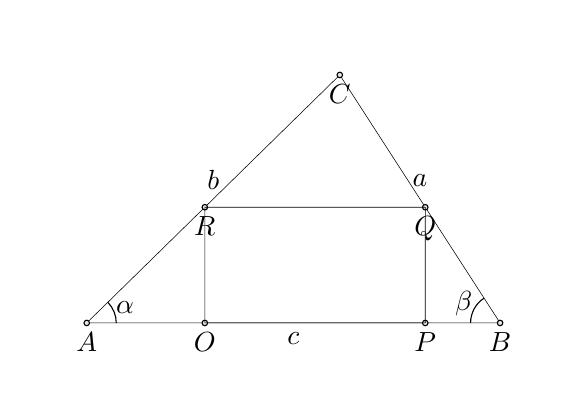
\begin{tikzpicture}[scale=0.75]

      \tkzInit[xmax=8, xmin=-1, ymin=-1, ymax=5]
      \tkzClip

      \tkzDefPoint(0,0){A}
      \tkzDefPoint(7,0){B}
      \tkzInterCC[R](A,6cm)(B,5cm)
      \tkzGetPoints{C}{D}
      \tkzDrawPolygon(A,B,C)
      \tkzLabelSegment[below](A,B){$c$}
      \tkzLabelSegment[above](A,C){$b$}
      \tkzLabelSegment[above=1pt](B,C){$a$}

      \tkzDefPoint(2,0){O}
      \tkzDefPoint(2,-1){o}
      \tkzInterLL(O,o)(A,C)\tkzGetPoint{R}
      \tkzDefLine[parallel=through R](A,B) \tkzGetPoint{r}

      \tkzInterLL(R,r)(B,C)\tkzGetPoint{Q}

      \tkzDefLine[parallel=through Q](R,O) \tkzGetPoint{P}
      \tkzDrawPoints(A,B,C,O,R,Q,P)
      \tkzDrawPolygon(O,P,Q,R)
      \tkzLabelPoints(A,B,C,O,R,Q,P)

\tkzMarkAngle[size=0.5](B,A,C)
\tkzLabelAngle[pos=0.7](B,A,C){$\alpha$}

\tkzMarkAngle[size=0.5](C,B,A)
\tkzLabelAngle[pos=0.7](C,B,A){$\beta$}
    \end{tikzpicture}
  \end{figure}

  \emph{Soln:} By cosine rule, we know that
  \begin{align*}
    \cos \alpha = \frac{ b^2+c^2-a^2}{2bc}=\frac{5}{7}, \cos \beta = \frac{ a^2+c^2-b^2}{2ac} = 19/35.
  \end{align*}

  Suppose that $OR = QP = h$, then
  \begin{align*}
    OP = c - AO - PB = c - \left(\frac{1}{\tan\alpha}+\frac{1}{\tan\beta}\right)h.
  \end{align*}

  Therefore, the area is
  \begin{align*}
    Area = (7-1.667 h ) h . 
  \end{align*}
  This is a quadratic polynomial with roots $0,\,4.199$. Hence, the maximum is achieved when $h = (0+4.199)/2$ and the maximum is 7.349.
\newpage
\item The points $A$, $B$, $C$, and $D$ are illustrated in figure below. An engineer wants to use a curve to connect the segment $AB$ and $CD$ and make the connection as smooth as possible. Design a quadratic Bezier curve to achieve this task and find the quadratic equation describing the curve.

  \begin{figure}[ht]
    \centering
    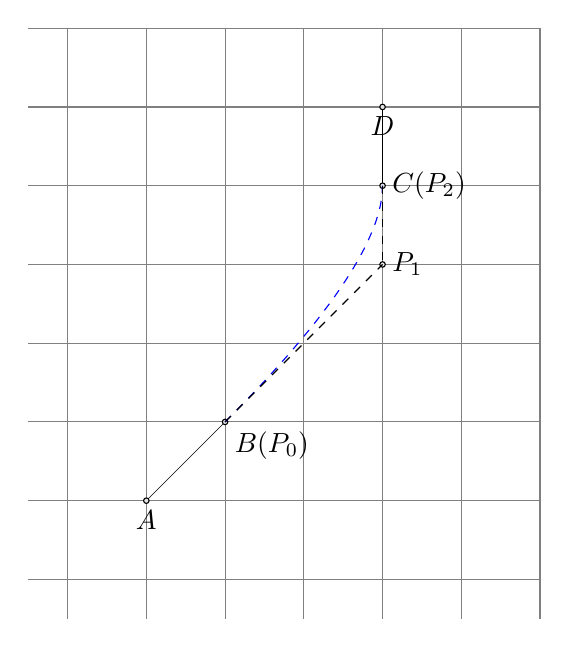
\begin{tikzpicture}
      \tkzInit[xmax=6, xmin=-0.5, ymin=-0.5, ymax=7]
      \tkzAxeXY
      \tkzGrid
      \tkzClip
      \tkzDefPoint(1,1){A}
      \tkzDefPoint[label=-45:{$B(P_0)$}](2,2){B}
      \tkzDefPoint[label=0:{$C(P_2)$}](4,5){C}
      \tkzDefPoint(4,6){D}
      \tkzDefPoint[label=right:{$P_1$}](4,4){P}
      \tkzDrawSegments(A,B C,D)
      \tkzDrawPoints(A,B,C,D,P)

      \tkzLabelPoints(A,D)
      \draw[domain=0:1, samples=10,smooth,variable=\t,dashed,blue,] plot ({-2*\t*\t+4*\t+2},{-\t*\t+4*\t+2});
      \draw[dashed](B)--(P);
      \draw[dashed](C)--(P);
    \end{tikzpicture}
  \end{figure}

  \emph{Soln:} Since the curve starts at $B$ and ends at $C$, we know $P_0 = B$ and $P_2 = C$. To make the curve smooth, $AB$ and $CD$ are both tangent lines of the curve and hence $P_1 =(4,4) $. The parametric equation for Bezier curve is
  \begin{align*}
    x &= 2(1-t)^2 + 8t(1-t)+4t^2 = -2t^2+4t+2  \\
    y &= 2(1-t)^2 + 8t(1-t)+5t^2 = -t^2+4t+2.
  \end{align*}
  Therefore, $t = (2y-x-2)/4$ and quadratic equation is given by
  \begin{align*}
   x^2-4xy+4y^2+20x-24y+4=0. 
  \end{align*}
\newpage
\item Find the standard form of the quadratic equation $3x^2 - 2xy + 3y^2 + 20x -12y +32 = 0.$

  \emph{Soln:} We can compute $\Delta_1 = 6,\,\Delta_2 = 8$ and $\Delta_3 = -32$. As a result, the equation represents either an ellipse or a hyerbola, which can be transformed into
  \begin{align*}
    Ax^2+Cy^2+F = 0,
  \end{align*}
  with
  \begin{align*}
    A +C=6,\,AC=8,\,ACF = -32.
  \end{align*}
  Therefore, $A = 2$, $C = 4$ and $F = -4$, which leads to the following standard form of an ellipse:
  \begin{align*}
    \frac{1}{2}x^2+y^2=1.
  \end{align*}



\newpage
\item A driver is driving along a straight highway and she is observing a mountain at point $E$ far away. She first drives $1$km from $A$ to $B$ and observe the apparent shift of $E$ is $\angle AEB = 10^\circ$. She then drives another $2$km and observe the apparent shift of $E$ is $\angle BEC = 20^\circ$. Calculate the distance from $E$ to the highway.

  \begin{figure}[ht]
    \centering
    \begin{tikzpicture}[scale=0.8]
    \tkzInit[xmax=7, xmin=-1, ymin=-1, ymax=12]
      \tkzClip
      \tkzDefPoint(0,0){A}
      \tkzDefPoint(2,0){B}
      \tkzDefPoint(6,0){C}

      \coordinate (p) at (0,{2*tan(80)});
      \coordinate (q) at (2,{4*tan(70)});

      \tkzDefCircle[circum](A,B,p)

      \tkzGetPoint{pp}

      \tkzDefCircle[circum](B,C,q)
      \tkzGetPoint{qq}

      \tkzInterCC(pp,A)(qq,B)
      \tkzGetPoints{E}{F}
      \tkzDrawPoints(A,B,C,E)
      \tkzLabelPoints(A,B,C,E)

      \tkzDrawPolygon(A,C,E)

      \tkzDrawSegment(B,E)

    \end{tikzpicture}
  \end{figure}

  \emph{Soln:} In $\triangle EAB$ and $\triangle EBC$, we have
  \begin{align*}
    \frac{EA}{\sin \angle EBA} = \frac{AB}{\sin 10^\circ}, \frac{EC}{\sin \angle EBC} = \frac{BC}{\sin 20^\circ}.
  \end{align*}
  Since $\sin \angle EBC = \sin \angle EBA$, we have
  \begin{align*}
    \frac{EA}{EC} = \frac{AB/\sin 10^\circ}{BC/\sin 20^\circ} = 0.9848.
  \end{align*}
  Now use the cosine rule in $\triangle EAC$:
  \begin{align*}
    EA^2+ EC^2 - 2EA\times EC\cos 30^\circ=AC^2.
  \end{align*}
  Hence, we can solve $EA = 5.749$ and $EC = 5.838$. Now use the sine rule in $\triangle EAC$, we get
  \begin{align*}
   \sin A = \frac{EC}{AC}\sin 30^\circ.
  \end{align*}
  The distance of $E$ to the line $AC$ is
  \begin{align*}
    EA \sin A = \frac{EA\times EC}{AC}\sin 30^\circ = 5.593.
  \end{align*}

\newpage




\item The orbit of a comet is a conic curve with eccentricity $1.25$. When the comet is at the perihelion point, its distance to the sun is $d$ and its speed is $v$. Calculate the speed of the comet $v'$ when it is $2.25d$ away from the sun.

  \emph{Soln:} Suppose the hyperbola is in the standard form
  \begin{align*}
    \frac{x^2}{a^2} - \frac{y^2}{b^2} = 1,
  \end{align*}
  with the Sun at $(c,0)$. The perihelion point of the comet corresponds to the vectex $(a,0)$. Therefore $c-a = d$. On the other hand, $e = c/a = 1.25$. Therefore,
  \begin{align*}
    c=5d,\, a = 4d,\,b = \sqrt{c^2-a^2} = 3d.
  \end{align*}
  The hyperbola takes the form:
  \begin{align}
    \frac{x^2}{16} - \frac{y^2}{9} = d^2.
    \label{eq:hyperbola}
  \end{align}


  The directrix of the hyperbola is at $x = a/e = 3.2d$. Suppose at point $P$, the distance of the comet to the sun is $2.25d$. Then the distance of the comet to the directrix is $x-3.2d = 2.25d/e$, which means $x = 5d$ and $y  = 2.25d$ from \eqref{eq:hyperbola}.

  The tangent line of the hyperbola at point $P$ is
  \begin{align*}
    \frac{5}{16}x - \frac{2.25}{9}y = 1.
  \end{align*}
  Therefore, the slope is $5/16\times 9/2.25 = 1.25$, Since $PF$ is parallel to the $y$-axis, the angle between $PF$ and the direction of the velocity is $90^\circ + \tan ^{-1}(1.25) = 141.34^\circ$. Now by Kepler's second law
  \begin{align*}
   \frac{1}{2}v\times VF \sin 90^\circ = \frac{1}{2} v' \times  PF \sin 141.34^\circ\Rightarrow v' = 0.711v.
  \end{align*}

   \begin{figure}[ht]
    \centering
    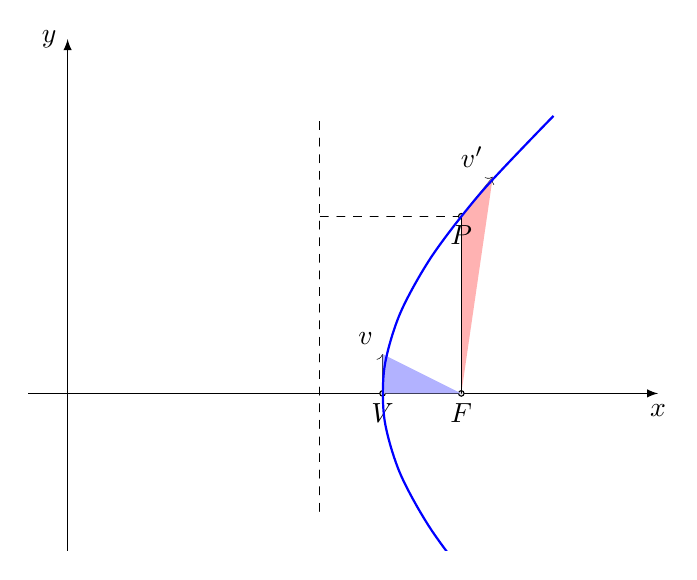
\begin{tikzpicture}

      \tkzInit[xmax=7, xmin=-0.5, ymin=-2, ymax=4]
      \tkzDrawX
      \tkzDrawY
      \tkzClip

      \tkzDefPoint(5,0){F}
      \tkzDefPoint(4,0){V}
      \tkzDefPoint(5,2.25){P}

      \tkzDefPoint(3.2,-1.5){A}
      \tkzDefPoint(3.2,3.5){B}

      \tkzDefPoint[label=135:{$v'$}](5.4,2.75){PP}
      \tkzDefPoint[label=135:{$v$}](4,0.5){VV}

      \tkzDefPointBy[projection=onto A--B](P)
      \tkzGetPoint{p}

      \tkzDrawSegment[dashed](A,B)
      \tkzDrawSegment[dashed](P,p)
      \tkzDrawSegment[->](P,PP)
      \tkzDrawSegment[->](V,VV)

      \tkzDrawPoints(F,V,P) 
      \tkzFillPolygon[red!30](F,P,PP) 

      \tkzFillPolygon[blue!30](F,V,VV) 

      \tkzDrawSegments(P,F)
      \tkzLabelPoints(P,F,V)
      \draw[domain=-1:1, samples=10,smooth,variable=\t,blue,thick] plot ({4*cosh(\t)},{3*sinh(\t)});
    \end{tikzpicture}
  \end{figure}

  
\end{enumerate}

\end{document}
%%% Local Variables:
%%% TeX-command-default: "Latexmk"
%%% End:

